\section{Analysis}

\begin{frame}
    \frametitle{Protocols}

    Our analysis shows that XMPP traffics experience longer latency than HTTP(s).

    \vskip 1em
    \centering
    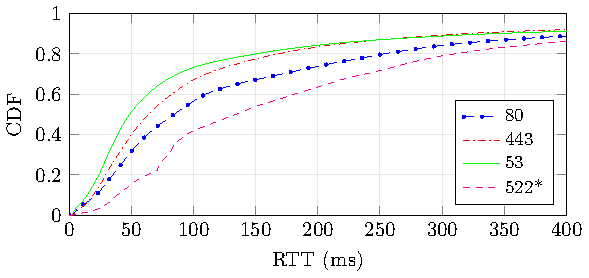
\includegraphics[width=.65\textwidth]{fig/port_performance.pdf}

    % 5222, 5223 and 5224 are used by XMPP, which is a common protocol for IM and VoIP services.
\end{frame}

\begin{frame}
    \frametitle{DNS Performance\footnote{servers deployed IP Anycast are considered ``diff country'' in this chapter}}

    % We know DNS is a criticle part of todays internet, and it's performance has great impacts on the QoE
    Users using DNS server that are located on different countries experience longer latency to app servers. This suggests the need for IP Anycasting.

    \vskip 1em
    \begin{columns}
        \begin{column}{.5\textwidth}
            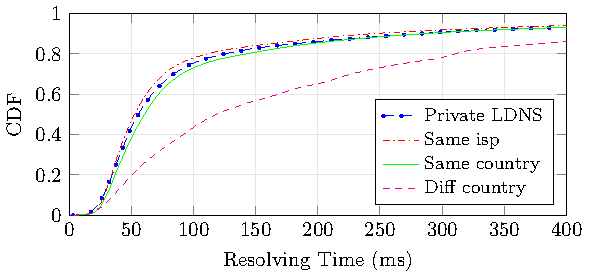
\includegraphics[width=\textwidth]{fig/dns_performance.pdf}
        \end{column}

        \begin{column}{.5\textwidth}
            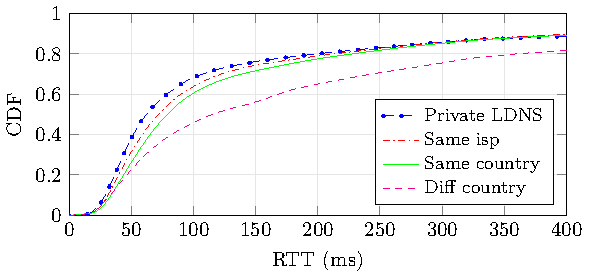
\includegraphics[width=\textwidth]{fig/dns_overall.pdf}
        \end{column}
    \end{columns}
\end{frame}

\begin{frame}
    \frametitle{IP Anycast}
    We identify Anycast IP using the the list conducted by iGreedy.\footnote{https://anycast.telecom-paristech.fr/dataset/}
    We use rlm() from R package MASS with default parameters to perform robust regression.

    \vskip 1em
    \centering
    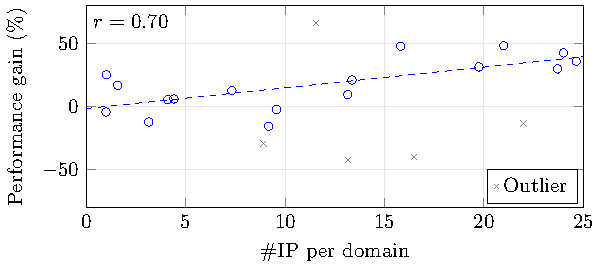
\includegraphics[width=.65\textwidth]{fig/anycast_nip_per_domain.pdf}
\end{frame}

\begin{frame}
    \frametitle{Application Servers}
    \centering
    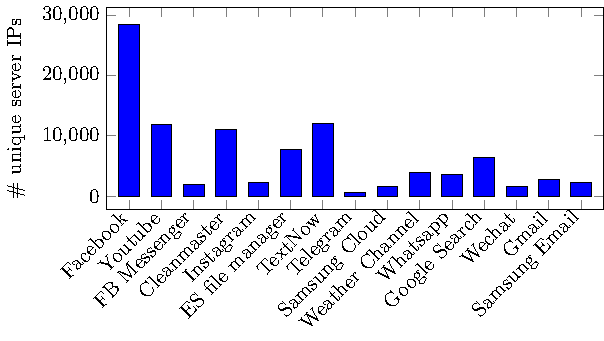
\includegraphics[width=.65\textwidth]{fig/server_number.pdf}
\end{frame}

\begin{frame}
    \frametitle{Application Servers}
    The Ad servers and trackers are identified by EasyList.\footnote{https://easylist.to/}

    \vskip .6em
    \centering
    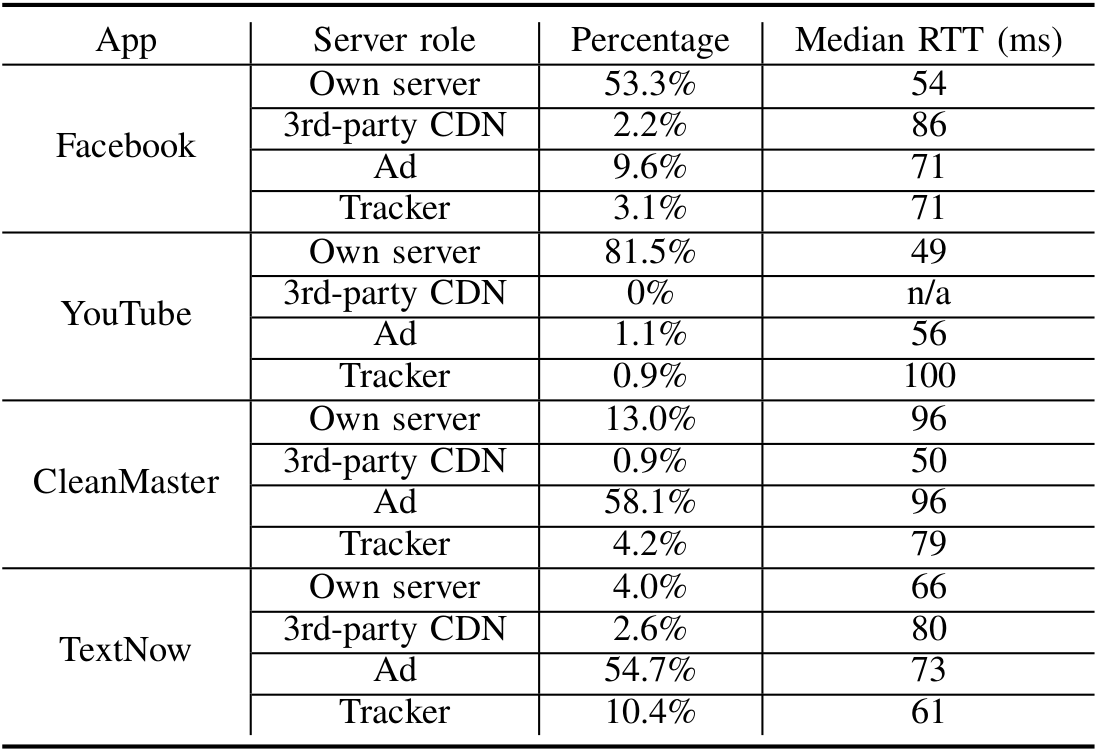
\includegraphics[width=.52\textwidth]{fig/table.png}
\end{frame}
